% ShareWise domain proposal: manually laid out, editable TikZ figure.
% Compile with: pdflatex -halt-on-error ShareWise-service-boundaries.tex
\documentclass[tikz,border=0pt]{standalone}
\usepackage[T1]{fontenc}
\usepackage{sourcesanspro}
\usepackage{tikz}
\usetikzlibrary{arrows.meta}
\definecolor{Ink}{HTML}{17233B}
\definecolor{Muted}{HTML}{52647A}
\definecolor{Rule}{HTML}{D7DFE8}
\definecolor{IAMBg}{HTML}{F1F5FC}
\definecolor{IAMLine}{HTML}{8BA8CC}
\definecolor{IAMStrong}{HTML}{365E90}
\definecolor{GroupBg}{HTML}{EFF9F5}
\definecolor{GroupLine}{HTML}{85B5A6}
\definecolor{GroupStrong}{HTML}{2E796B}
\definecolor{ExpenseBg}{HTML}{FFF8EA}
\definecolor{ExpenseLine}{HTML}{DCB978}
\definecolor{ExpenseStrong}{HTML}{916421}
\definecolor{SettleBg}{HTML}{F5F1FB}
\definecolor{SettleLine}{HTML}{AB91CC}
\definecolor{SettleStrong}{HTML}{745393}
\tikzset{
  outerbox/.style={line width=.9pt,rounded corners=4.5pt},
  event/.style={line width=1.8pt,densely dashed,-{Stealth[length=7pt,width=6pt]}},
  smalllabel/.style={font=\sffamily\fontsize{9}{11}\selectfont,text=Muted},
  bodylabel/.style={font=\sffamily\fontsize{10}{12}\selectfont,text=Ink},
  eventlabel/.style={font=\sffamily\fontsize{10}{12}\selectfont,text=Ink,fill=white,inner sep=2.5pt},
}
\begin{document}
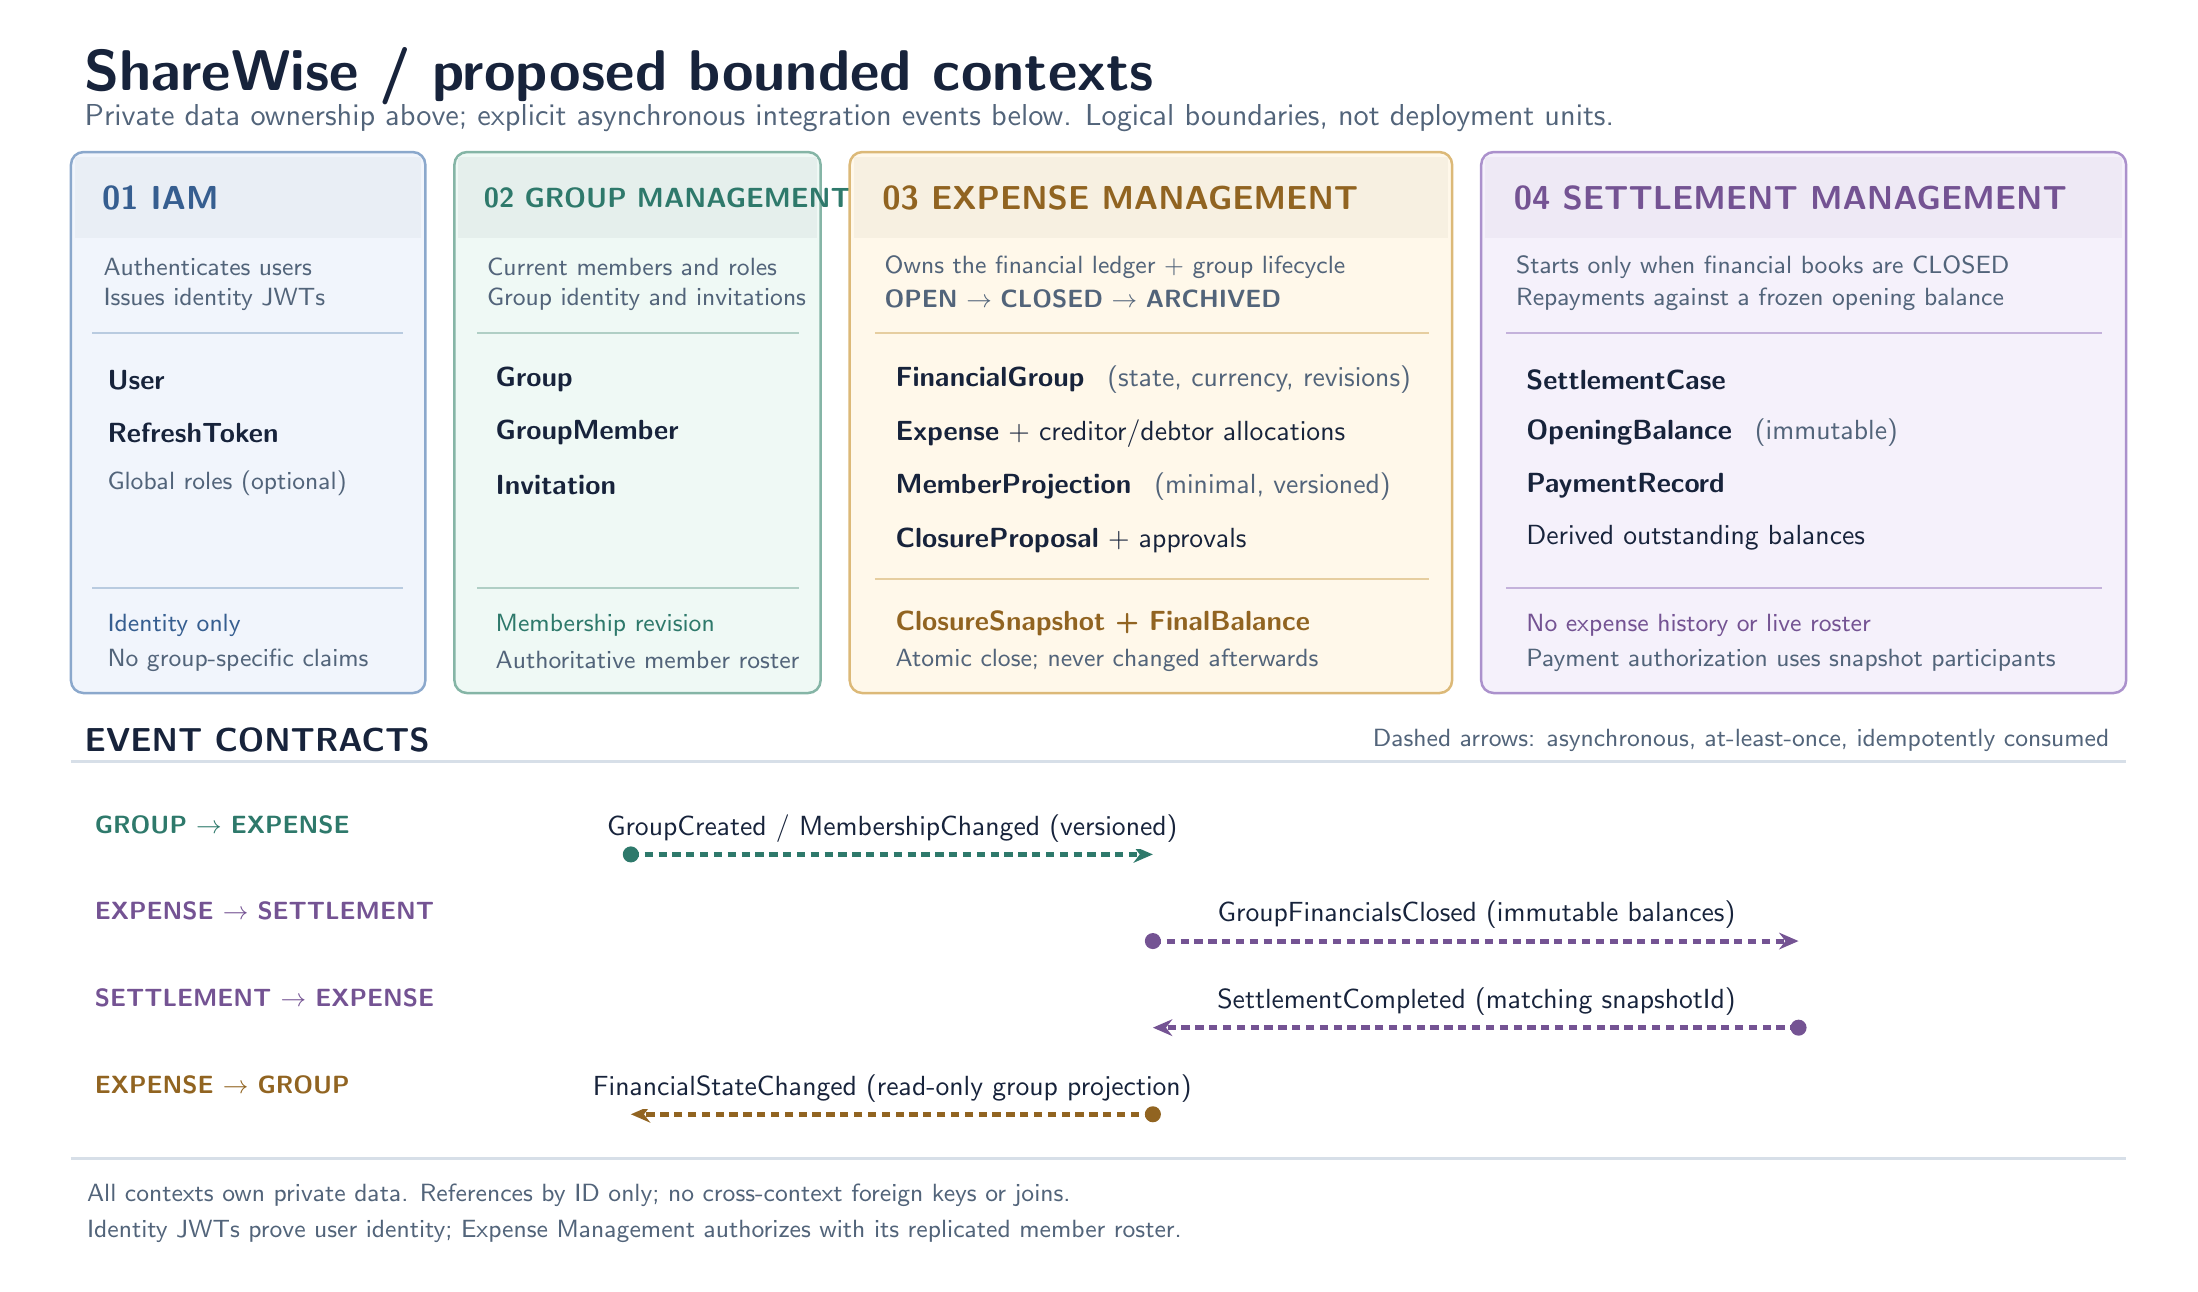
\begin{tikzpicture}[x=1cm,y=1cm]
  \path[use as bounding box] (0,0) rectangle (27.20,15.70);
  % Title and short explanation.
  \node[anchor=west,font=\sffamily\bfseries\fontsize{20}{24}\selectfont,text=Ink]
    at (.60,15.08) {ShareWise  /  proposed bounded contexts};
  \node[anchor=west,font=\sffamily\fontsize{10.5}{12}\selectfont,text=Muted]
    at (.60,14.55) {Private data ownership above; explicit asynchronous integration events below. Logical boundaries, not deployment units.};

  % ===================== Bounded context cards =====================
  % Identity
  \draw[outerbox,draw=IAMLine,fill=IAMBg] (.55,7.25) rectangle (5.05,14.12);
  \fill[fill=IAMLine!19] (.60,13.03) rectangle (5.00,14.06);
  \node[anchor=west,font=\sffamily\bfseries\fontsize{12}{14}\selectfont,text=IAMStrong] at (.82,13.54) {01  IAM};
  \node[anchor=west,smalllabel] at (.84,12.66) {Authenticates users};
  \node[anchor=west,smalllabel] at (.84,12.25) {Issues identity JWTs};
  \draw[draw=IAMLine!60,line width=.65pt] (.82,11.82) -- (4.77,11.82);
  \node[anchor=west,bodylabel] at (.89,11.23) {\textbf{User}};
  \node[anchor=west,bodylabel] at (.89,10.56) {\textbf{RefreshToken}};
  \node[anchor=west,smalllabel] at (.89,9.92) {Global roles (optional)};
  \draw[draw=IAMLine!60,line width=.65pt] (.82,8.58) -- (4.77,8.58);
  \node[anchor=west,font=\sffamily\fontsize{9.5}{11}\selectfont,text=IAMStrong] at (.89,8.11) {Identity only};
  \node[anchor=west,smalllabel] at (.89,7.67) {No group-specific claims};

  % Group Management
  \draw[outerbox,draw=GroupLine,fill=GroupBg] (5.42,7.25) rectangle (10.07,14.12);
  \fill[fill=GroupLine!21] (5.47,13.03) rectangle (10.02,14.06);
  \node[anchor=west,font=\sffamily\bfseries\fontsize{9.8}{12}\selectfont,text=GroupStrong] at (5.67,13.54) {02  GROUP MANAGEMENT};
  \node[anchor=west,smalllabel] at (5.71,12.66) {Current members and roles};
  \node[anchor=west,smalllabel] at (5.71,12.25) {Group identity and invitations};
  \draw[draw=GroupLine!65,line width=.65pt] (5.71,11.82) -- (9.79,11.82);
  \node[anchor=west,bodylabel] at (5.82,11.23) {\textbf{Group}};
  \node[anchor=west,bodylabel] at (5.82,10.56) {\textbf{GroupMember}};
  \node[anchor=west,bodylabel] at (5.82,9.89) {\textbf{Invitation}};
  \draw[draw=GroupLine!65,line width=.65pt] (5.71,8.58) -- (9.79,8.58);
  \node[anchor=west,font=\sffamily\fontsize{9.5}{11}\selectfont,text=GroupStrong] at (5.82,8.11) {Membership revision};
  \node[anchor=west,smalllabel] at (5.82,7.67) {Authoritative member roster};

  % Expense Management
  \draw[outerbox,draw=ExpenseLine,fill=ExpenseBg] (10.44,7.25) rectangle (18.09,14.12);
  \fill[fill=ExpenseLine!22] (10.49,13.03) rectangle (18.04,14.06);
  \node[anchor=west,font=\sffamily\bfseries\fontsize{12}{14}\selectfont,text=ExpenseStrong] at (10.73,13.54) {03  EXPENSE MANAGEMENT};
  \node[anchor=west,smalllabel] at (10.76,12.66) {Owns the financial ledger + group lifecycle};
  \node[anchor=west,smalllabel] at (10.76,12.25) {\textbf{OPEN}  $\rightarrow$  \textbf{CLOSED}  $\rightarrow$  \textbf{ARCHIVED}};
  \draw[draw=ExpenseLine!70,line width=.65pt] (10.76,11.82) -- (17.80,11.82);
  \node[anchor=west,bodylabel] at (10.90,11.23) {\textbf{FinancialGroup}  \hspace{.5em}\textcolor{Muted}{(state, currency, revisions)}};
  \node[anchor=west,bodylabel] at (10.90,10.55) {\textbf{Expense} + creditor/debtor allocations};
  \node[anchor=west,bodylabel] at (10.90,9.87) {\textbf{MemberProjection} \hspace{.5em}\textcolor{Muted}{(minimal, versioned)}};
  \node[anchor=west,bodylabel] at (10.90,9.19) {\textbf{ClosureProposal} + approvals};
  \draw[draw=ExpenseLine!70,line width=.65pt] (10.76,8.70) -- (17.80,8.70);
  \node[anchor=west,font=\sffamily\bfseries\fontsize{10}{12}\selectfont,text=ExpenseStrong] at (10.90,8.13) {ClosureSnapshot + FinalBalance};
  \node[anchor=west,smalllabel] at (10.90,7.67) {Atomic close; never changed afterwards};

  % Settlement Management
  \draw[outerbox,draw=SettleLine,fill=SettleBg] (18.46,7.25) rectangle (26.65,14.12);
  \fill[fill=SettleLine!20] (18.51,13.03) rectangle (26.60,14.06);
  \node[anchor=west,font=\sffamily\bfseries\fontsize{12}{14}\selectfont,text=SettleStrong] at (18.75,13.54) {04  SETTLEMENT MANAGEMENT};
  \node[anchor=west,smalllabel] at (18.78,12.66) {Starts only when financial books are CLOSED};
  \node[anchor=west,smalllabel] at (18.78,12.25) {Repayments against a frozen opening balance};
  \draw[draw=SettleLine!70,line width=.65pt] (18.78,11.82) -- (26.34,11.82);
  \node[anchor=west,bodylabel] at (18.91,11.23) {\textbf{SettlementCase}};
  \node[anchor=west,bodylabel] at (18.91,10.56) {\textbf{OpeningBalance} \hspace{.5em}\textcolor{Muted}{(immutable)}};
  \node[anchor=west,bodylabel] at (18.91,9.89) {\textbf{PaymentRecord}};
  \node[anchor=west,bodylabel] at (18.91,9.22) {Derived outstanding balances};
  \draw[draw=SettleLine!70,line width=.65pt] (18.78,8.58) -- (26.34,8.58);
  \node[anchor=west,font=\sffamily\fontsize{9.5}{11}\selectfont,text=SettleStrong] at (18.91,8.11) {No expense history or live roster};
  \node[anchor=west,smalllabel] at (18.91,7.67) {Payment authorization uses snapshot participants};

  % ===================== Horizontal event lanes =====================
  \node[anchor=west,font=\sffamily\bfseries\fontsize{12}{14}\selectfont,text=Ink]
    at (.60,6.65) {EVENT CONTRACTS};
  \node[anchor=east,font=\sffamily\fontsize{9.5}{11}\selectfont,text=Muted]
    at (26.56,6.65) {Dashed arrows: asynchronous, at-least-once, idempotently consumed};
  \draw[draw=Rule,line width=.9pt] (.55,6.38) -- (26.65,6.38);

  % Dedicated tracks: each event has its own horizontal lane, never overlaps another.
  % Group -> Expense
  \node[anchor=west,font=\sffamily\bfseries\fontsize{9.3}{11}\selectfont,text=GroupStrong] at (.73,5.57) {GROUP $\rightarrow$ EXPENSE};
  \draw[event,draw=GroupStrong] (7.66,5.20) -- (14.29,5.20);
  \node[eventlabel,anchor=south] at (10.98,5.26) {GroupCreated  /  MembershipChanged (versioned)};
  % Expense -> Settlement
  \node[anchor=west,font=\sffamily\bfseries\fontsize{9.3}{11}\selectfont,text=SettleStrong] at (.73,4.48) {EXPENSE $\rightarrow$ SETTLEMENT};
  \draw[event,draw=SettleStrong] (14.29,4.10) -- (22.49,4.10);
  \node[eventlabel,anchor=south] at (18.40,4.16) {GroupFinancialsClosed  (immutable balances)};
  % Settlement -> Expense
  \node[anchor=west,font=\sffamily\bfseries\fontsize{9.3}{11}\selectfont,text=SettleStrong] at (.73,3.38) {SETTLEMENT $\rightarrow$ EXPENSE};
  \draw[event,draw=SettleStrong] (22.49,3.00) -- (14.29,3.00);
  \node[eventlabel,anchor=south] at (18.40,3.06) {SettlementCompleted  (matching snapshotId)};
  % Expense -> Group
  \node[anchor=west,font=\sffamily\bfseries\fontsize{9.3}{11}\selectfont,text=ExpenseStrong] at (.73,2.28) {EXPENSE $\rightarrow$ GROUP};
  \draw[event,draw=ExpenseStrong] (14.29,1.90) -- (7.66,1.90);
  \node[eventlabel,anchor=south] at (10.98,1.96) {FinancialStateChanged  (read-only group projection)};

  % Legend dots under relevant context columns to identify source and destination.
  \foreach \x/\y/\col in {7.66/5.20/GroupStrong,14.29/4.10/SettleStrong,22.49/3.00/SettleStrong,14.29/1.90/ExpenseStrong} {
    \fill[\col] (\x,\y) circle[radius=2.9pt];
  }
  \draw[draw=Rule,line width=.9pt] (.55,1.34) -- (26.65,1.34);
  \node[anchor=west,font=\sffamily\fontsize{9.5}{11.5}\selectfont,text=Muted]
    at (.63,.87) {All contexts own private data. References by ID only; no cross-context foreign keys or joins.};
  \node[anchor=west,font=\sffamily\fontsize{9.5}{11.5}\selectfont,text=Muted]
    at (.63,.42) {Identity JWTs prove user identity; Expense Management authorizes with its replicated member roster.};
\end{tikzpicture}
\end{document}
